\section{Features}

A more extensive list of search features can be shown using the \texttt{--help}
switch.

\subsection{Search Algorithms}
\label{sub:Search Algorithms}

The solver implements the following search methods:

\begin{itemize}
  \item Uninformed
  \begin{itemize}
    \item Breadth-First Search, \texttt{BFS}
    \item Depth-First Search, \texttt{DFS}
    \item Iterative-Deepening Depth First Search (IDDFS), \texttt{IDS,CUS1}
    \item Bogosort Search, \texttt{BOGO,CUS3}
  \end{itemize}
  \item Informed:
  \begin{itemize}
    \item Greedy Best-First Search, \texttt{GBFS}
    \item A* Search, \texttt{AS}
    \item Iterative-Deepening A-Star Search (IDA*), \texttt{IDAS,CUS2}
  \end{itemize}
\end{itemize}

\subsubsection{Thresholds}
\label{subs:Thresholds}

IDDFS and IDA* searches can utilise the \texttt{--threshold}
switch when executing, which will specify the initial maximum node path cost, or
$pc(n)$, to traverse, for IDS, or the limit to the evaluation function
result, $f(n)$, that will be accepted for searches, for \texttt{IDAS}).
That is, for a threshold of $t$, the following:
\begin{align}\label{eq:thresholds}
  pc(n) < t_{\text{IDDFS}}\\
  f(n) < t_{\text{IDA*}}
\end{align}

As these are iterative depth searches, the initial threshold is \emph{doubled}
each time nodes are calculated to no longer be within the current threshold.
These nodes are temporarily stored in a \emph{fallback} frontier and are used
only if there are no more nodes to search for, thereby initialising the next
\emph{iteration}. Refer to Section~\ref{sub:Search Traversal} for more detail.

\subsubsection{Heuristics}
\label{subs:Heuristics}

By default, the heuristic used for informed searches is the Manhattan Distance
heuristic, shown below in Equiation \ref{eq:manhattan}. The distance of state,
$s$, of an $n$ by $m$ puzzle is calculated by the sum of the absolute
differences of a tile $t$'s coordinates from the state to it's goal state,
$\bar{s}$.

\begin{equation} \label{eq:manhattan}
  h(s)_{\text{manhattan}} =
    \sum_{t=1}^{n \times m} \ ( \
      | \ x_{t}(s) - x_{t}(\bar{s}) \ | \ + \ | \ y_{t}(s) - y_{t}(\bar{s}) \ |
    \ )
\end{equation}

Similarly, the Chebyshev and Euclidean Distances are also avaliable for
heuristics calculation. See \ref{eq:chebyshev} and \ref{eq:euclidean},
respectively. The last avaliable heuristic is the misplaced tiles count,
which is simply the number of mismatches in the position tiles

\begin{equation} \label{eq:chebyshev}
  h(s)_{\text{chebyshev}} =
    \sum_{t=1}^{n \times m} \ ( \
      \mathbf{max}( \ | \ x_{t}(s) - x_{t}(\bar{s}) \ | \ , \ | \ y_{t}(s) - y_{t}(\bar{s}) \ | \ )
    \ )
\end{equation}

\begin{equation} \label{eq:euclidean}
  h(s)_{\text{euclidean}} =
    \sum_{t=1}^{n \times m} \ ( \
      \sqrt{ ( \ x_{t}(s) - x_{t}(\bar{s}) \ )^{2} + ( \ y_{t}(s) - y_{t}(\bar{s}) \ )^{2} }
    \ )
\end{equation}

The heuristic used on an informed search can be changed to other heuristics by
using the  \texttt{--heuristic} switch and providing one of: \texttt{manhattan},
\texttt{euclidean}, \texttt{manhattan}, \texttt{chebyshev} or
\texttt{misplaced}. Refer to the help for more instructions.

\subsection{Graphical Solver}
\label{sub:Graphical Solver}

A graphical solver can show both the search method solving the puzzle
as well as a solution to the puzzle where state's in the node tree are
represented by the $n$ by $m$ matrix as coloured tiles. See Figure~\ref{fig:gui}.

\begin{figure}[h!]
  \centering
  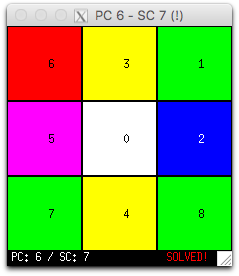
\includegraphics{gui.png}
  \caption{GUI of a puzzle solver}
  \label{fig:gui}
\end{figure}

The GUI can be initiated using the following switches:

\begin{itemize}
  \item \texttt{\bfseries --gui=solved}
  Show only the solved puzzle. Traverse the search tree from the root node to
  the goal node using the \texttt{B} or $\uparrow$ Keys and down the tree using
  the \texttt{F} or $\downarrow$ Keys
  \item \texttt{\bfseries --gui=solving}\footnote{Note that when using the
  solving GUI, the search algorithm may appear to be slower than when not using
  the GUI. This is due to render lag caused by X11, used to render the GUI.}
  Show the search algorithm solving the puzzle. When solving the GUI will not be
  responsive, so should the solver need to be quit, termination at the command
  line using \texttt{\^{}C} is required
\end{itemize}
